\documentclass[dvipsnames]{beamer}
\input{mybeamerdefs}

\begin{document}

\begin{frame}{\today}
\begin{itemize}
\item I looked into the distortion from the metabolic image of 2019-12-12 based on the BW per pixel and frequency offset between metabolites.
\item I tested the execution time of the 2DFT sequence on Supershop.
\item I implemented diffusion for the ems.
\item I wrote a script to generate a DWI pulse sequence.
\item I simulated em diffusion + a DWI sequence.
\end{itemize}
\end{frame}

\section{Distortion from metabolic image}

\begin{frame}{Summary}
\begin{itemize}
\item I found the BW per pixel to be 125 Hz.
\item I found the frequency offset to be -1277 Hz.
\item \begin{equation*} \mathrm{int}\left(\frac{-1277 Hz}{125 Hz} \right) = -10\end{equation*}
\item Take a look at the image.
\end{itemize}
\end{frame}

\begin{frame}{Image from 2019-12-12}
\begin{center}
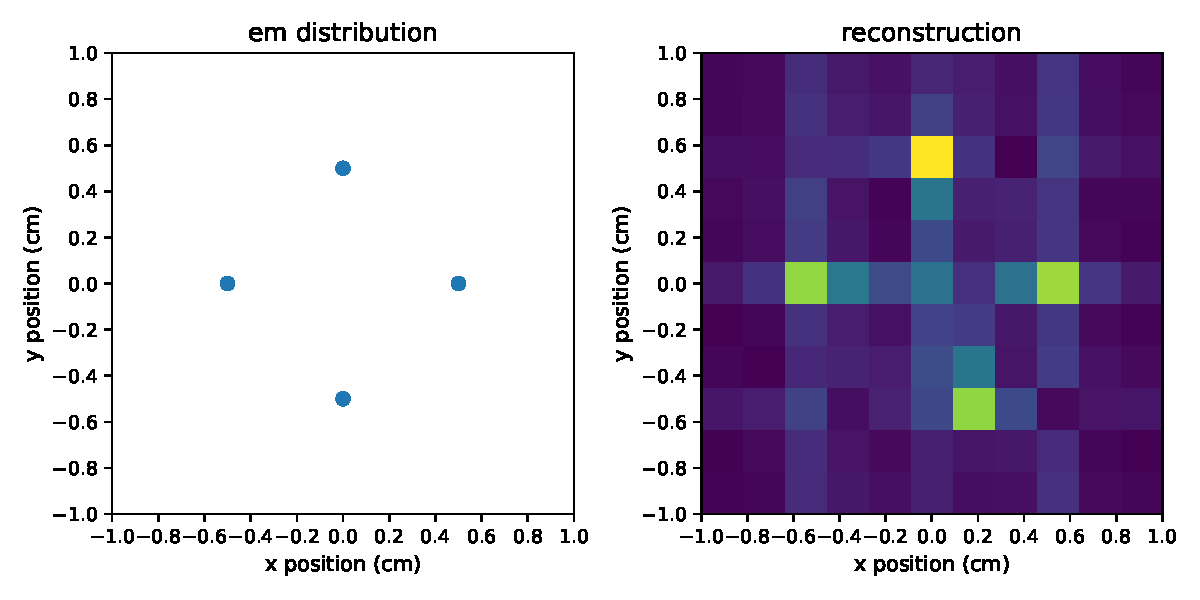
\includegraphics[width=\textwidth]{reconstruction_metabolism-on-20percent}
\end{center}
\end{frame}

\begin{frame}{Comments}
\begin{itemize}
\item The bottommost em is shifted 10 pixels to the left (if you wrap around to the other side of the image). Checks out!
\end{itemize}
\end{frame}

\section{Execution time of 2DFT sequence on Supershop}

\begin{frame}{Summary}
\begin{itemize}
\item I ran the same script as 2019-12-12 for testing the execution time on Supershop.
\item The total execution time was 129.8 seconds.
\item This means 129.8 microseconds per em per time step.
\end{itemize}
\end{frame}

\begin{frame}{Comments}
\begin{itemize}
\item Why is the execution time so much slower on Supershop than on my Macbook? The execution time on my Macbook was 5.41 microseconds per em per time step.
\end{itemize}
\end{frame}

\section{Em diffusion}

\begin{frame}{Summary}
\begin{itemize}
\item I looked into diffusion simulation methods.
\item I implemented diffusion in the Em class.
\item I instantiated one em and took $10^4$ diffusion steps and plotted the trajectory.
\end{itemize}
\end{frame}

\begin{frame}{Simulating diffusion}
\begin{itemize}
\item Assume space is isotropic.
\item Let $D(x,y,z)$ be the diffusion coefficient at position $(x,y,z)$.
\item Let $\Delta t$ be the time step of the simulation.
\item Update the position of each em as
\begin{equation*}
\begin{aligned}
x &\leftarrow x + Q_1\\
y &\leftarrow y + Q_2\\
z &\leftarrow z + Q_3\,,
\end{aligned}
\end{equation*}
where $Q_i \sim \mathcal{N}(0,2D(x,y,z)\Delta t)$.
\end{itemize}
\end{frame}

\begin{frame}
\begin{itemize}
\item I am uncertain whether $Q_i \sim \mathcal{N}(0,2D(x,y,z)\Delta t)$ is correct or if it should be $Q_i \sim \mathcal{N}(0,D(x,y,z)\Delta t)$.
\item \href{https://arxiv.org/pdf/1212.0362.pdf}{This} reference says the former, \href{https://www.intechopen.com/books/theory-and-applications-of-monte-carlo-simulations/monte-carlo-simulation-of-particle-diffusion-in-various-geometries-and-application-to-chemistry-and-}{this} reference says the latter.
\item I am sticking with $Q_i \sim \mathcal{N}(0,2D(x,y,z)\Delta t)$ for now.
\end{itemize}

\end{frame}

\begin{frame}{Example trajectory of diffusing em}
\begin{center}
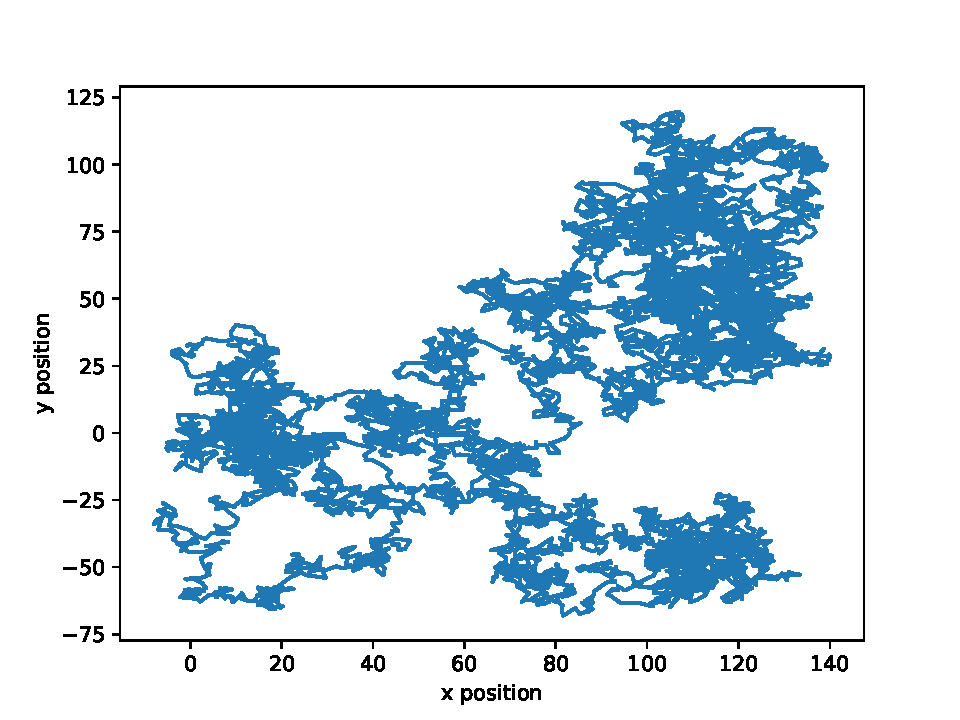
\includegraphics[height=0.8\textheight]{diffusion_trajectory}
\end{center}
\end{frame}

\begin{frame}{Comments}
\begin{itemize}
\item Trajectory looks reasonable.
\item The execution time for $10^4$ diffusion steps for a single em is 0.0783 seconds $\Rightarrow$ 7.828 microseconds per em per time step.
\item Compare with the 5.41 microseconds per em per time step of the 2DFT sequence simulation with stationary ems.
\item Generating the normally distributed random numbers required to model diffusion increases the computation time substantially.
\end{itemize}
\end{frame}

\section{DWI pulse sequence}

\begin{frame}{Summary}
\begin{itemize}
\item I modified the 2DFT sequence to produce a DWI sequence.
\item The user specifies the amplitude of the diffusion gradient in each of the 3 spatial directions, the duration of these diffusion gradients, and the time between the positive and negative lobes.
\item See the following figure for an example DWI sequence.
\end{itemize}
\end{frame}

\begin{frame}{DWI pulse sequence example}
\begin{center}
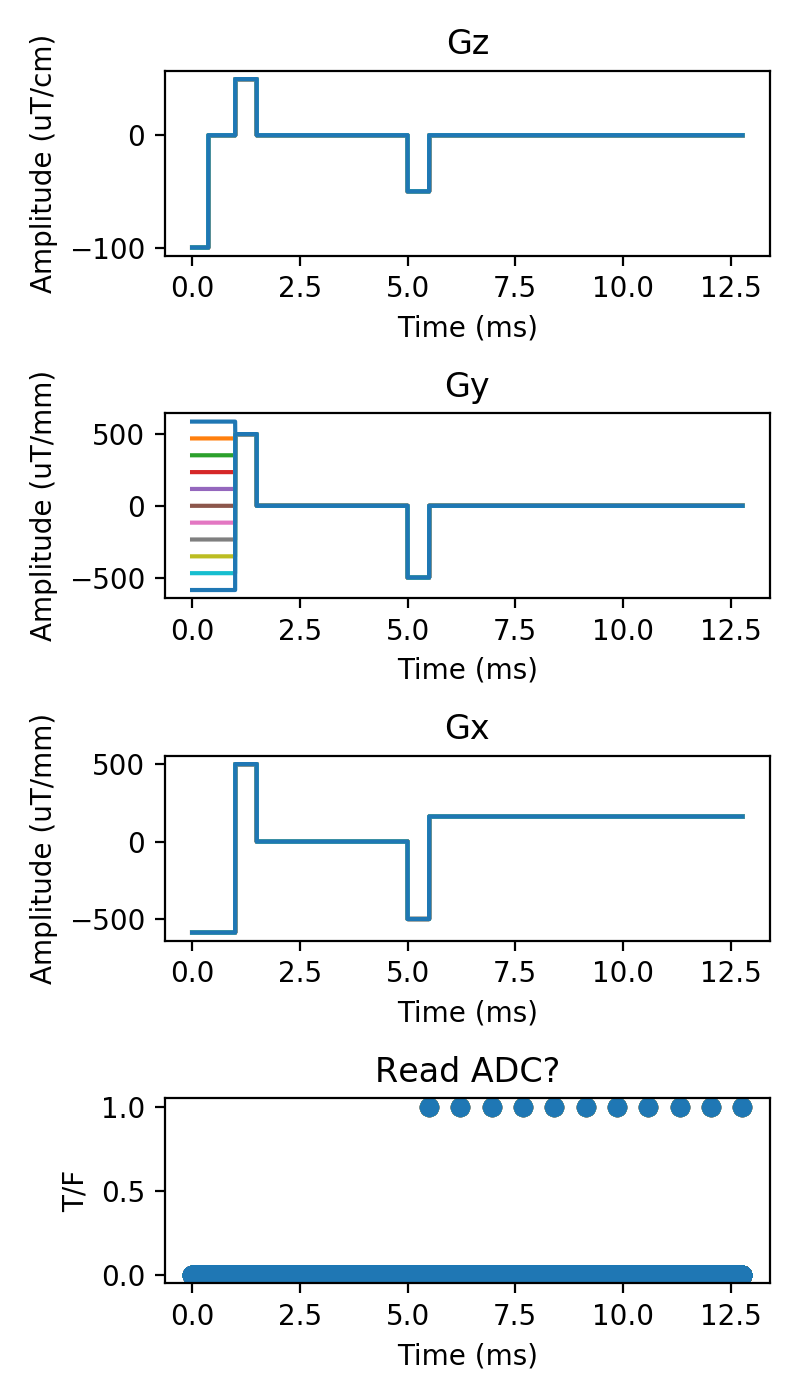
\includegraphics[height=0.8\textheight]{dwi_pulse_sequence.png}
\end{center}
\end{frame}

\begin{frame}{Comments}
\begin{itemize}
\item Does that look right?
\end{itemize}
\end{frame}

\section{DWI sequence simulation}

\begin{frame}{Summary}
\begin{itemize}
\item I defined the diffusion coefficient as $(D_x,D_y,D_z) = (5 \times 10^{-6}, \times 10^{-6},0)~\mathrm{m^2/s}$ for $x > 0$ and $(D_x,D_y,D_z) = (0,0,0)$ for $x <=0$.
\item I simulated a DWI sequence with diffusion gradients of $(5 \times 10^{-3},5 \times 10^{-3},5 \times 10^{-3})$ uT/cm, 1 ms diffusion gradient pulses, positive and negative lobes separated by 4 ms.
\end{itemize}
\end{frame}

\begin{frame}{Results}
\begin{center}
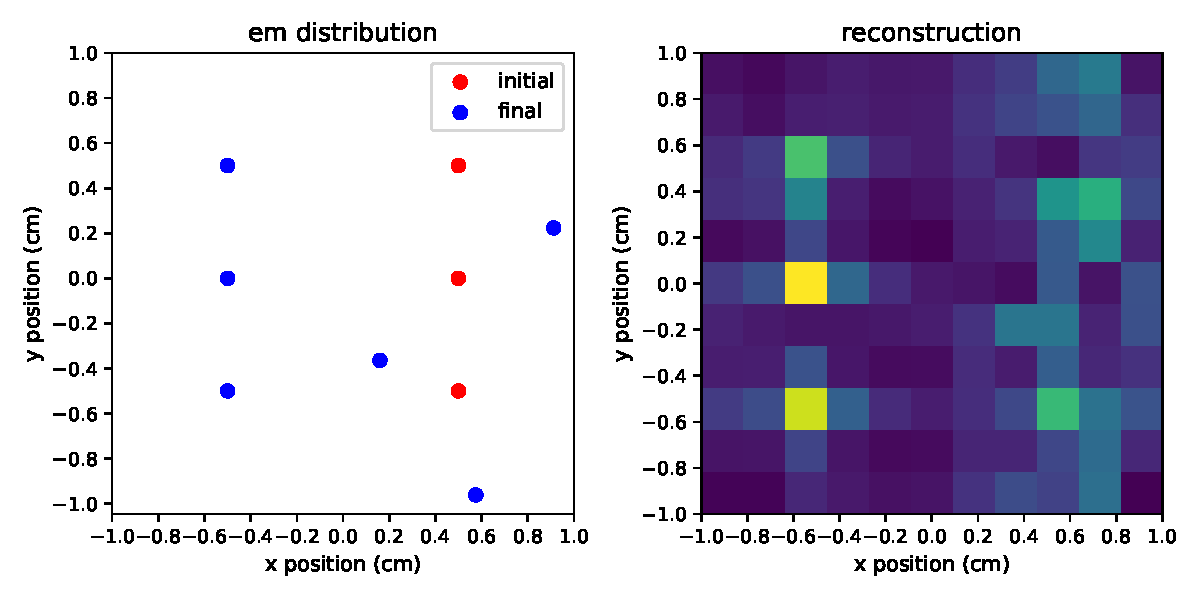
\includegraphics[width=\textwidth]{reconstruction_diffusion}
\end{center}
\end{frame}

\begin{frame}{Comments}
\begin{itemize}
\item The right side of the image (with a nonzero diffusion coefficient) is less intense than the left side (with zero diffusion coefficient).
\item It looks like the diffusion-weighting is working (?).
\end{itemize}
\end{frame}

\end{document}